\documentclass{article}
\usepackage[utf8]{inputenc}
\usepackage{graphicx}
\usepackage{float}

\usepackage{epsfig}
\usepackage{blindtext}
\usepackage{graphicx}
\usepackage[T1]{fontenc}
\usepackage{amsmath}



\title{MATH 444 PS3}
\author{Connor Wolfe cbw36 }
\date{March 10 2017}

\begin{document}

\maketitle

\section*{Core Algorithms}
\subsection*{Introduction}
This homework set tests two major topics: Linear Discriminant Analysis (LDA) and Alternating Nonlinear Least Squares (ANLS) algorithms.  I will begin by describing the algorithms I wrote for each, why they work, and how they are useful.  I will then analyze their implementations in problems 1 and 2.  
\subsection*{LDA}
\subsubsection*{Idea}
    LDA provides an improvement over visualizing data with PCA for the special case when we have clustered, annotated data. The LDA algorithm attempts to find a direction to project the data onto which will maximize the spread between the clusters (Sb) and minimize the spread within a cluster (Sw).  
\subsubsection*{Algorithm}function [V,D] = LDA (X,I)
        \begin{itemize}
            \item(lines 2-4) To begin, we caluclate preliminary values including the dimensions of X (n,p) and the number of clusters within X \\
        
            \item(lines 6-11) Next, we define a cell I\_c which will contain the annotation subvector for each cluster.  In other words, it will contain seperate vectors corresponding to the indices of all elements within each respective cluster and the number of elements in each cluster.  The operative code here is the find (I==i) function which finds all occurrences of i within the annotation vector. 
            
            \item(lines 16-20) Next we define a matrix c (n, \# clusters+1) which will store each luster centroids and the global centroid in the last index.  Finding the cluster centroid of cluster i is computed as follows:
            \\$c(:,i)=(1/I_c{i,2}) * sum(X(:,I==i),2);$\\
            This summing all of the elements in the cluster and dividing by the number of elements.
            
            \item(lines 23-26) Next we calculate X\_w which is the data vector X with each element centered about its cluster.  We do so by iterating through the number of clusters and subtracting each X by its cluster centroid.  The code to implement is the following:
            \\$X_w(:,I==i)=X(:,I==i)-c(:,i);$\\
            
            \item(line 29) We then calculate the within cluster scatter matrix Sw which represents the spread of the data within each cluster.  This is computed easily from the X\_w matrix calculated above, which makes sense because we just centered the data about its centroid. The Sw matrix is simply:
            \\$sw=X_w(:,:)*X_w(:,:)';$\\
            
            \item(lines 32-35) Finally, we calculate our last matrix Sb, the cluster scatter matrix.  This represents how spread each cluster is from one another.  We do this by finding how far each centroid is from the global center and weighting each centroids distance by its number of points.  This is calculated by summing all of the centroid distances from the global centroid.  The calculation of cluster i from the global center weighted by its length is shown below:
        \\$sb=sb+I_c{i,2}*(c(:,i)-c(:,num\_clusters+1))*(c(:,i)-c(:,num\_clusters+1))';$\\

            \item\textbf{REVISED} (Lines 38-41)  As we stated before, in order to find the best direction for projection, we want to maximize the Sb matrix and minimize the Sw matrix.  To do so at the same time, we find the eigenvector eigenvalue pair corresponding to the product of inv(Sw) and Sb.  This reads as:
            \\\begin{math}[V,D]=eigs(Sw\backslash Sb,2); \end{math}\\
            We must ensure both V and D are real in the following line.  Note the inclusion of '2' within the eigs function.  This says to take only the largest two directions, which is all we want for our graphing purposes.  
            
            \item(Lines 44-49)The final lines of the algorithm serve to plot the data about the directions we found above.  To do so, we calculate Z as the product of the transpose of the eigenvector maxtrix V and X.  We then plot the first row Z vs the second and color code according to cluster.  
            
            \item We will analyze the effectiveness of the algorithm on various data in the next sections.
        \end{itemize}
        
\subsection*{ANLS}
    \subsubsection*{Idea}
    The objective of the ANLS algorithm is to approximate $X^{nxp}$ by two vectors, $W^{nxk}$ and $H{kxp}$ with a measure of efficacy of the frobenius norm: $||X-WH||_F$ -->minimum.  To do so, we use a fixed point iteration algorithm, where we alternatively fix W and H, and find the other until convergance.  Note that the W norm is composed of dominant feature images and H is composed of coefficients which indicates how strongly an element in X is composed of this image.  
    \subsubsection*{Algorithm}
        \begin{itemize}
        \item Initialize (lines 8-14) set counter time=0, define tolerance t=0.01, and randomly initialize $W_{old}$ by $W_{old}=rand(256,k)$.
            
        \item {Iterate}\\
                A.  (Lines 18-21) Fix W and find the new H: \\$H_{new}(:,j)=lsqnonneg(W_{old},X(:,j));$\\
                
                B.  (Lines 24-26) Fix H and find the new W:         \\$W_{new}(i,:)=lsqnonneg(H_{new}',X(i,:)')';$\\
    
                C.  (Lines 29-32) We need to scale the matrices and choose to do so by the $l-\infty$ norm.  To do so, we define diagonal matrix L with lambda values:     
                $L(i,i)=max(W_{new}(:,i));$\\
                We scale the matrices as follows:
                \\$W_{new}=W_{new}L^{-1}$\\
                $H_{new}=LH_{new}$
                
                D.  (Lines 39-50) Check for convergence using the Frobenius norm.  We calculate the change in W by taking  $d||W||_F/||W||_F$ and the change in H as $d||H||_F/||H||_F$ (F for Frobenius norm).  We then compare q=dh+dw to the tolerance.  In order to calculate the Frobenius norm, I use the Matlab function: $norm(A,  'fro')$ which finds the Frobenius norm of A.
    
    
    \end{itemize}

\section*{Problem 1}
\subsection*{Introduction}
This problem analyzes the 'WineData.mat' file, which contains data set X (13x178) of chemical analysis of data of wines with three different cultivars (clusters) and annotation vector I (1x178) telling us to which cluster each X belongs to.  The task was to use the annotation of the data to find the best 3 directions for projections and to show/analyze how well the directions represent the clusters

\subsection*{Analysis}
    We can see in certain of the 3-direction plots and certainly in the 2-dimensional plot the clusters of the data.  It is worth noting that in some 3-direction plots, namely direction 2 vs 3 (lower left), or 2 vs 1 (upper right) the clustering is less clear.  However, in two directions, the clustering is extremely obvious.  The superiority of two dimensions comes from the fact that Z is calculated based off of V, and when we include lesser values in V (a third value of V that is, that is less than the first two) it dilutes the strength of V to cluster the data.  However, in certain 3-directional cases there is still obvious clustering, names 3 vs 1.   LDA performed well.

\subsection*{Data}

\begin{figure}[h!]
    \centerline
    {
    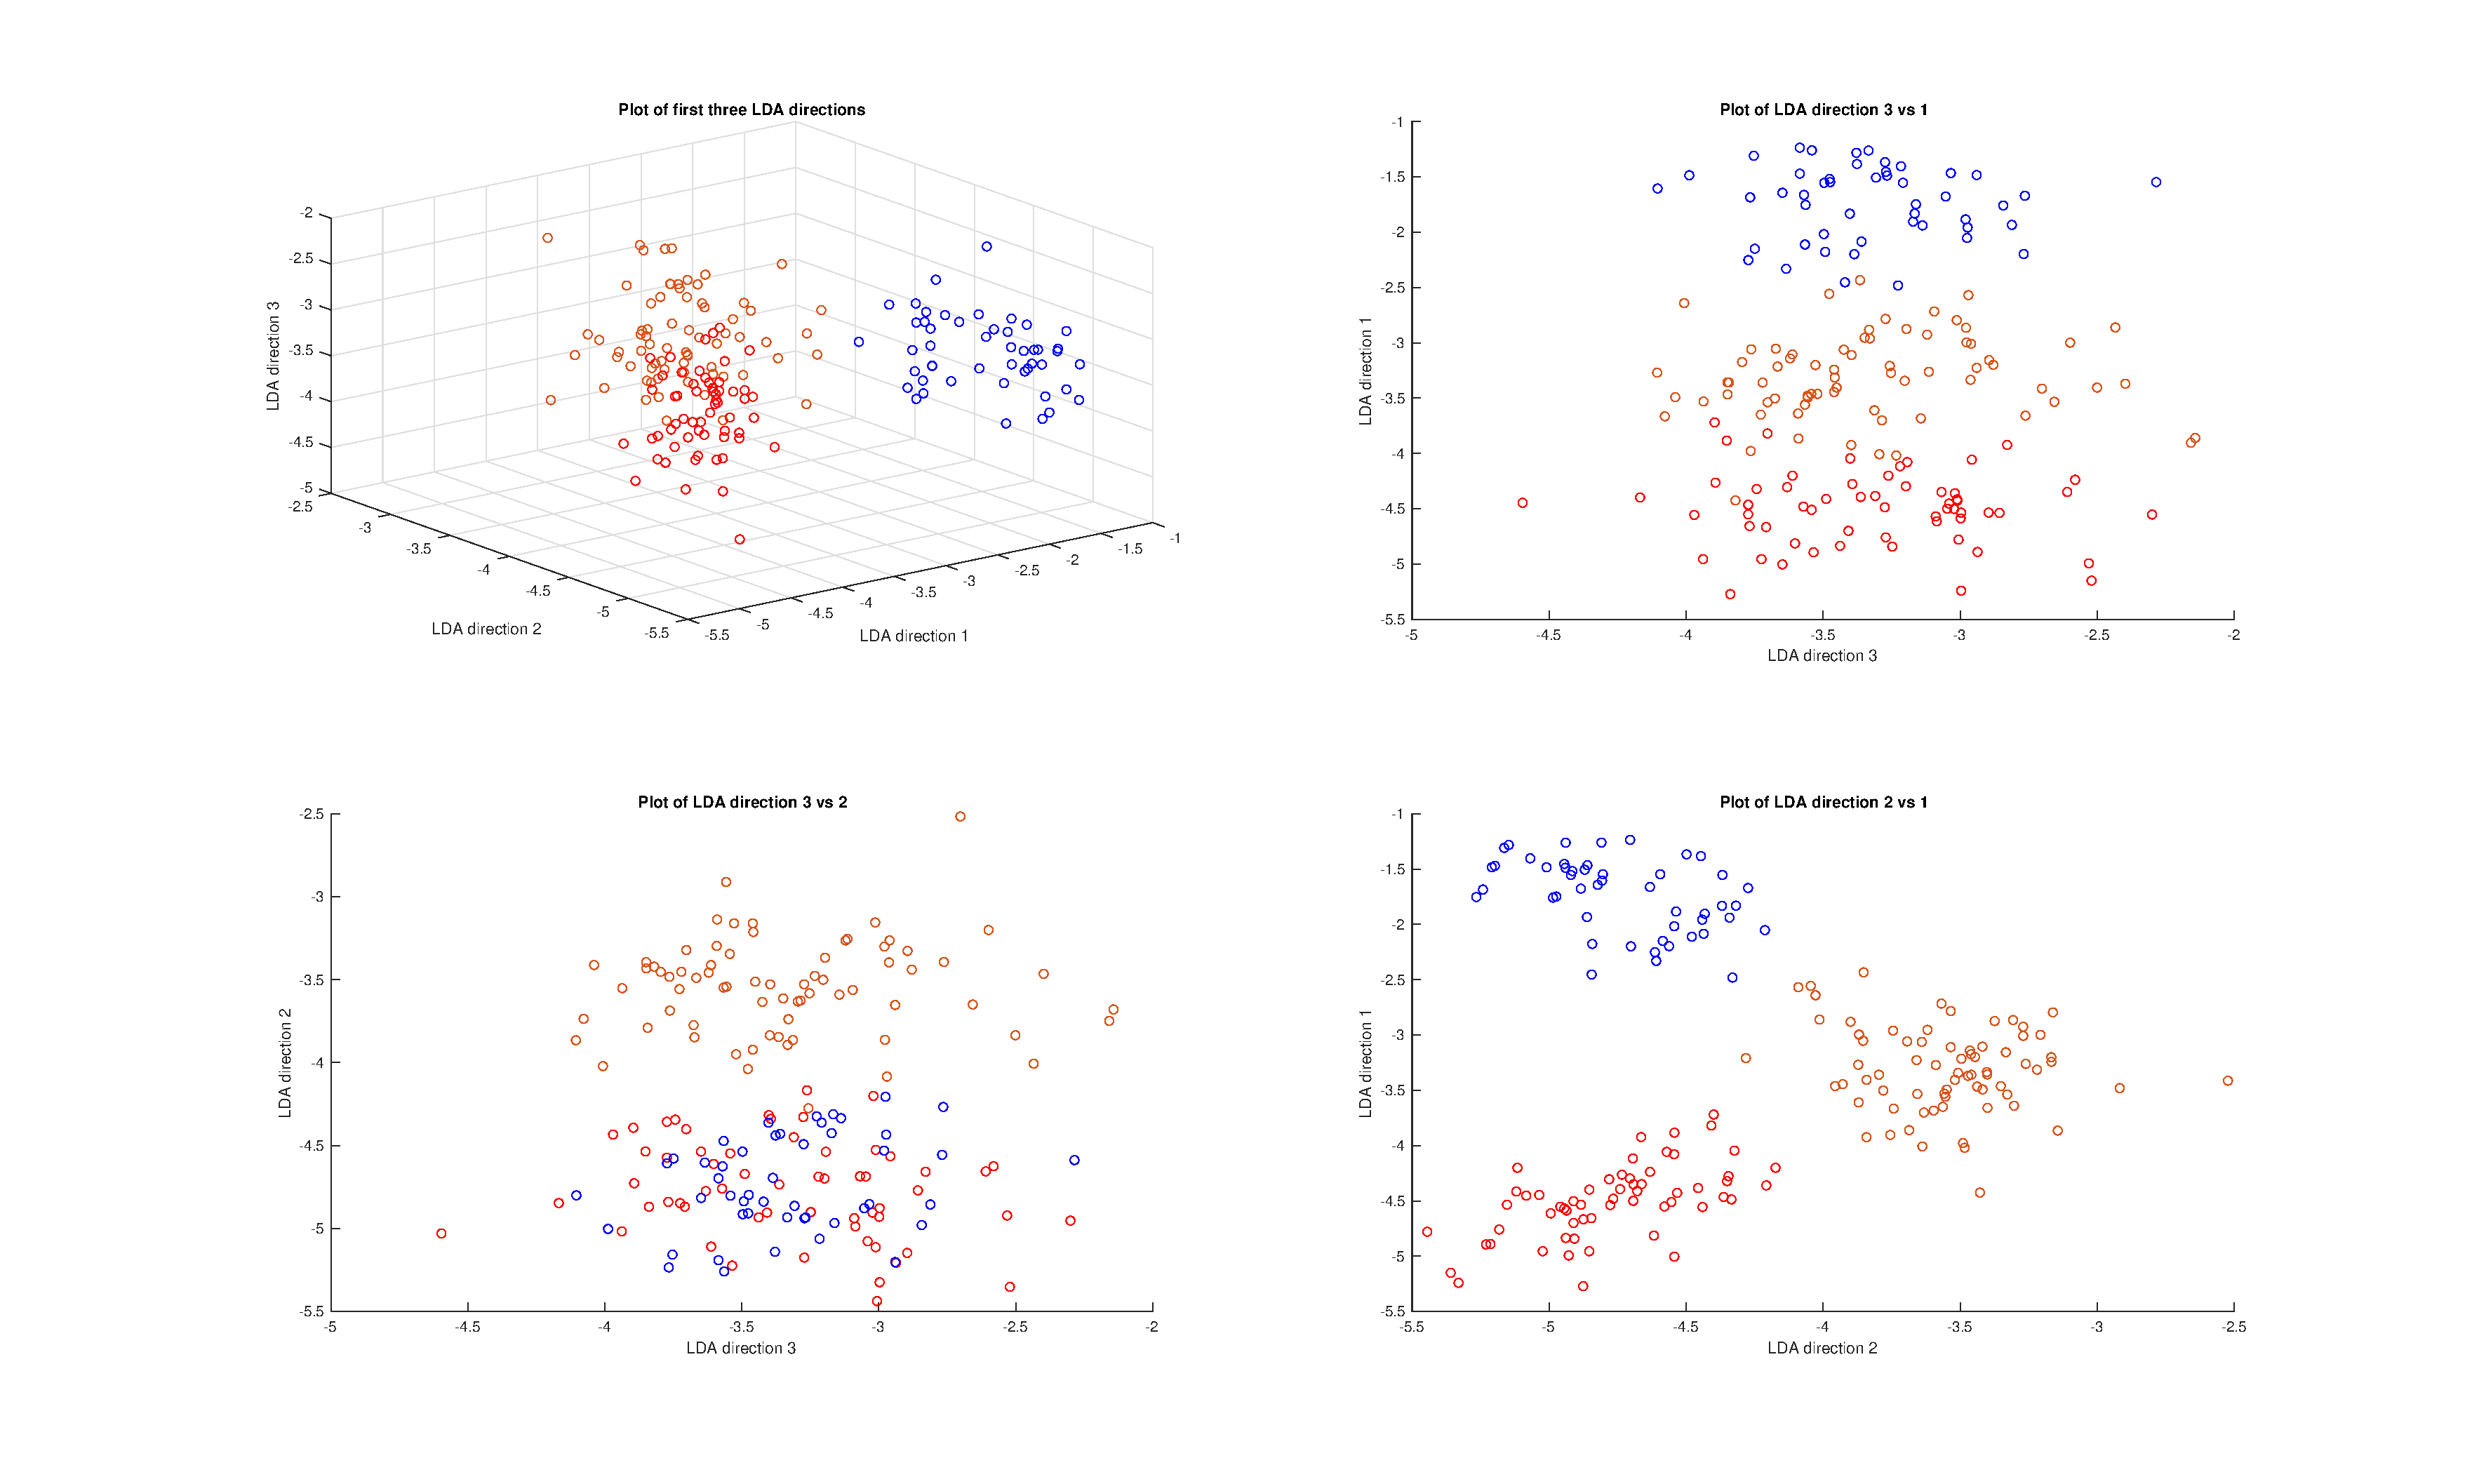
\includegraphics[width=20cm, height=10cm]{Q1_3LDA_Directions}
    }
    \caption{\label{fig:my figure} 4 different representations of the first 3 LDA directions of the wine data set.  The top left panel represents a 3-dimensional plot of them, and the remaining three represent the 3 permutations of the 3 directions}
\end{figure}

\begin{figure}[h!]
    \centerline
    {
    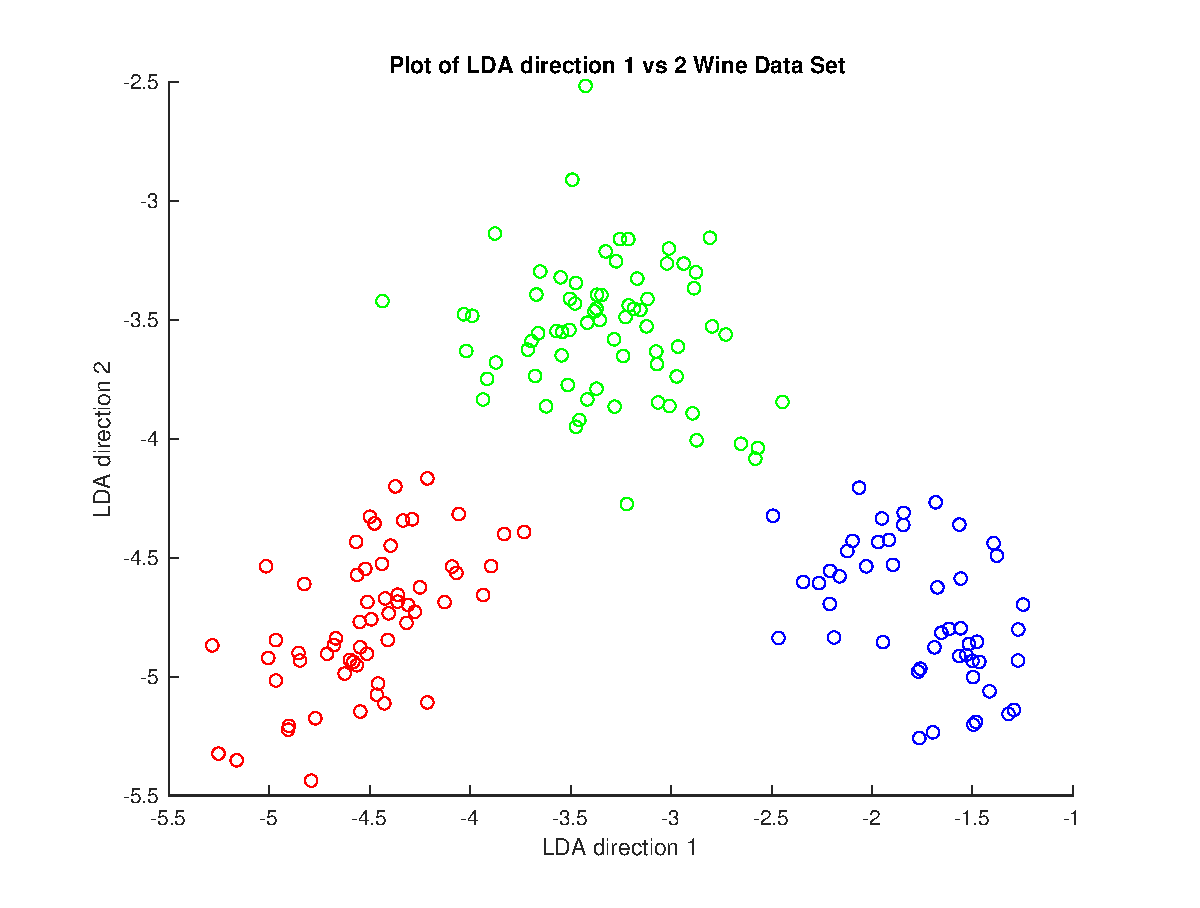
\includegraphics[width=20cm, height=10cm]{Q1_2LDA_Directions}
    }
    \caption{\label{fig:my figure} Plot of the first 2 LDA Directions on the wine data set }
\end{figure}


\section*{Problem 2}
\subsection*{Introduction}
The second problem works with the handwritten digits data set from problem sets prior.  We analyze the clustering and reconstruction of two digits, namely 0 and 4.\\
In part a, we will perform and LDA analysis on subset of X corresponding to the images 04 (call this matrix X04).  Then we plot the projection of X04 onto the first two LDA directions.  As I explain in my analysis, the clustering is not nearly as strong as in problem 1.  \\
In part b we will try to find the rank k=[5,10,20] factorization of X04 using the ANLS algorithm described previously.  We will plot the feature vectors from W as images and see pieces of 4's and 0's.   We will then see if the feature vectors that correspond to a 0 have coefficients in H that are large for 0 reconstructions and  small for 4 reconstructions.  I will then approximate X as WH and plot the reconstructions.  

\subsection*{Problem 2 (a)}
\subsubsection*{Data}
\begin{figure}[h!]
    \centerline
    {
    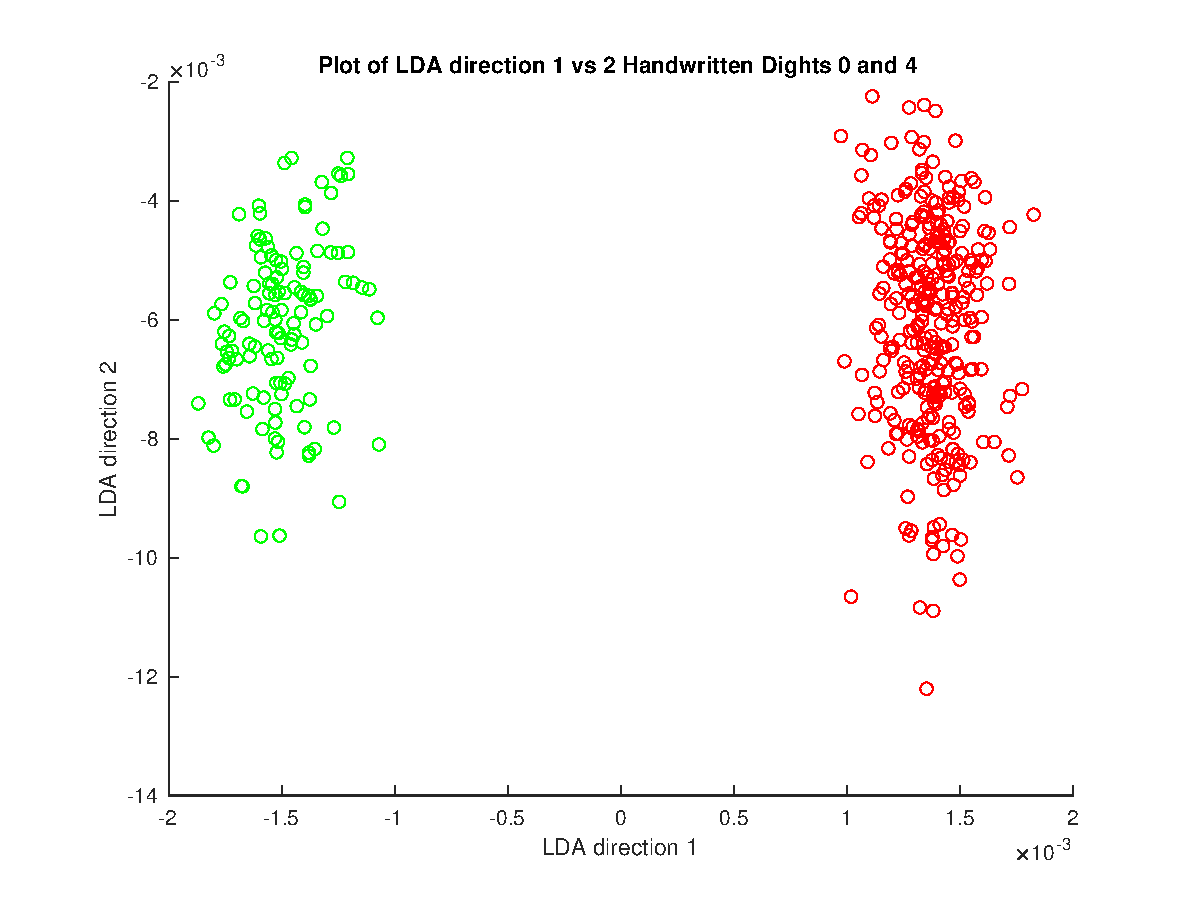
\includegraphics[width=15cm, height=10cm]{Q2_a_2LDA}}
    
    \caption{\label{fig:my figure} Plot of the first 2 LDA Directions of the handwritten data set for images of 0 and 4 only.  We can see the data clusters very well on the first direction and not very well on the second.}
\end{figure}
\subsubsection*{Analysis}
\textbf{REVISED} As expected, we are able to very well cluster the data for digits 0 and 4.  Note that in my previous submission I was unable to do so.  My correction was that I had a list of the cluster values 'cluster\_vals'=[0.4]. When I iterated through this array, I used the index of iteration (i=[1,2]) rather than the cluster\_value at that index. so I was searching for for data points corresponding to I=1 or 2 and yielding no points.  So I had empty arrays that I would operate with and had incorrect data.  The idea of the algorithm was correct, just the way I iterated that needed correction.  

\subsection*{Problem 2 (b)}
\subsubsection*{Data}

\begin{figure}[H]
    \centerline
    {
    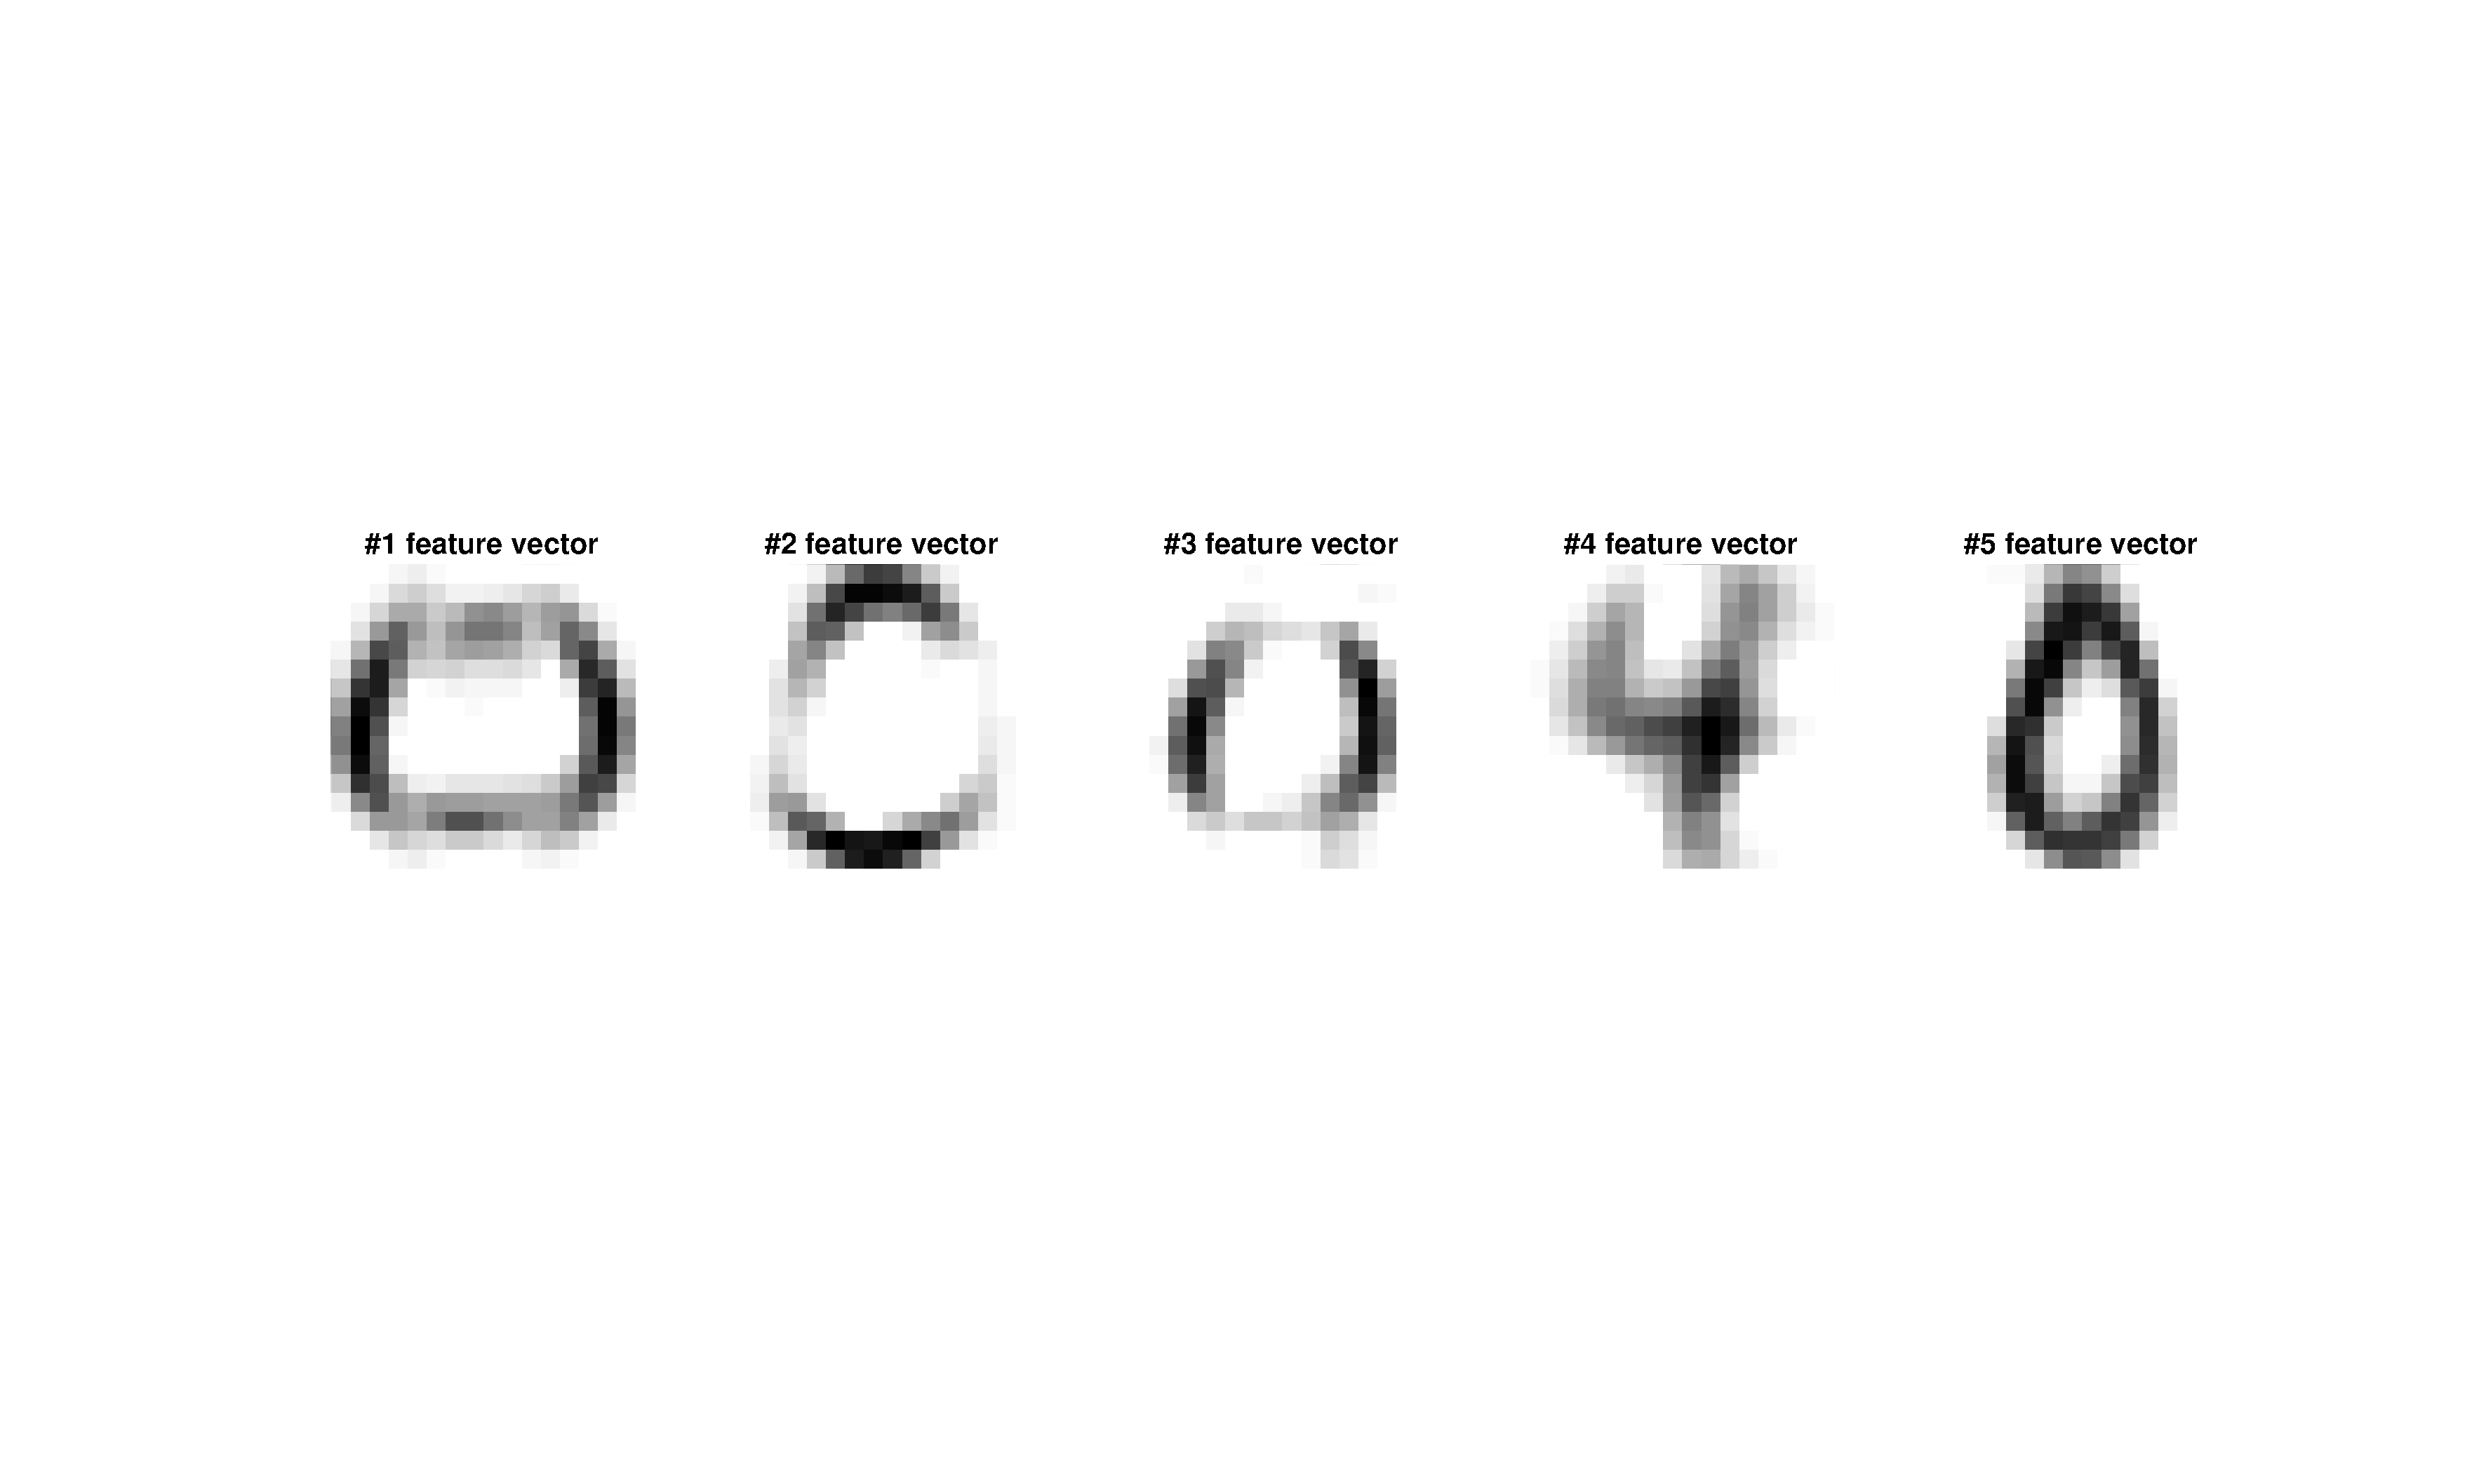
\includegraphics[width=10cm, height=7cm]{Q2_b_5FV}
    }
    \caption{\label{fig:my figure} Plot of the first 5 feature vectors of W from an ANLS run of X04.  Note all feature vectors clearly correspond to a 0 or a 4.}
\end{figure}

\begin{figure}[H]
    \centerline
    {
    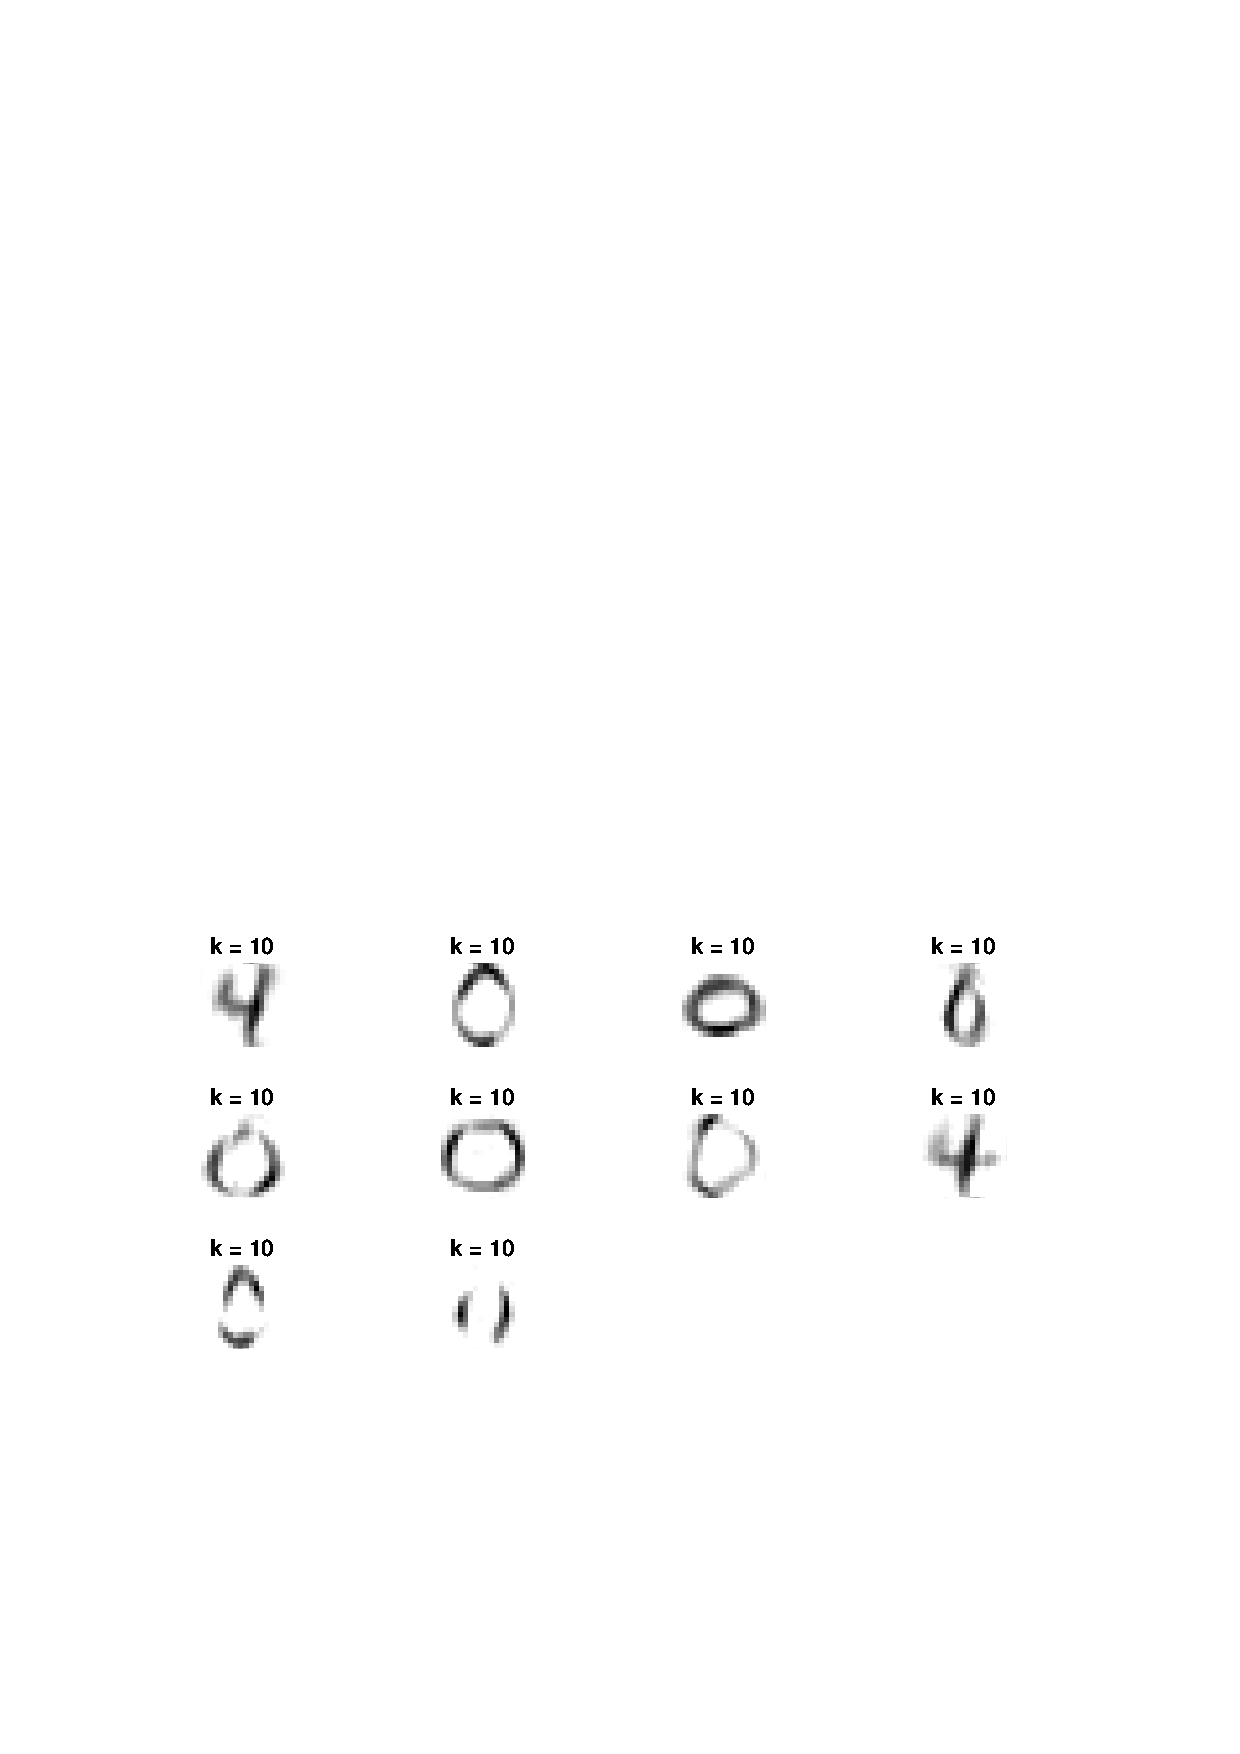
\includegraphics[width=10cm, height=7cm]{Q2_b_10FV}
    }
    \caption{\label{fig:my figure}\textbf{REVISED} Plot of the first 10 feature vectors of W from an ANLS run of X04.  Note all feature vectors clearly correspond to a 0 or a 4.}
\end{figure}

\begin{figure}[H]
    \centerline
    {
    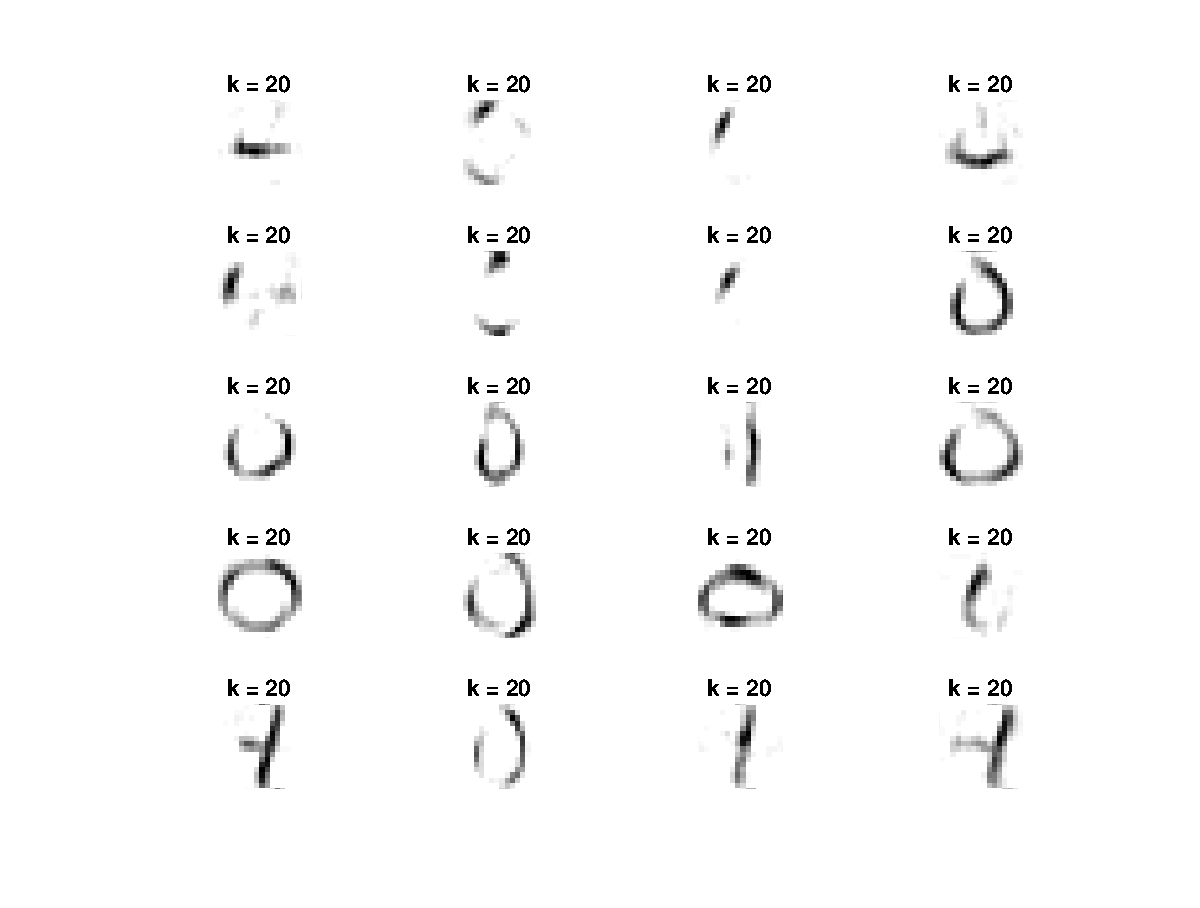
\includegraphics[width=10cm, height=8cm]{Q2_b_20FV}
    }
    \caption{\label{fig:my figure} \textbf{REVISED}Plot of the first 20 feature vectors of W from an ANLS run of X04.  Note all feature vectors clearly correspond to a 0 or a 4.}
\end{figure}

\begin{figure}[H]
    \centerline
    {
    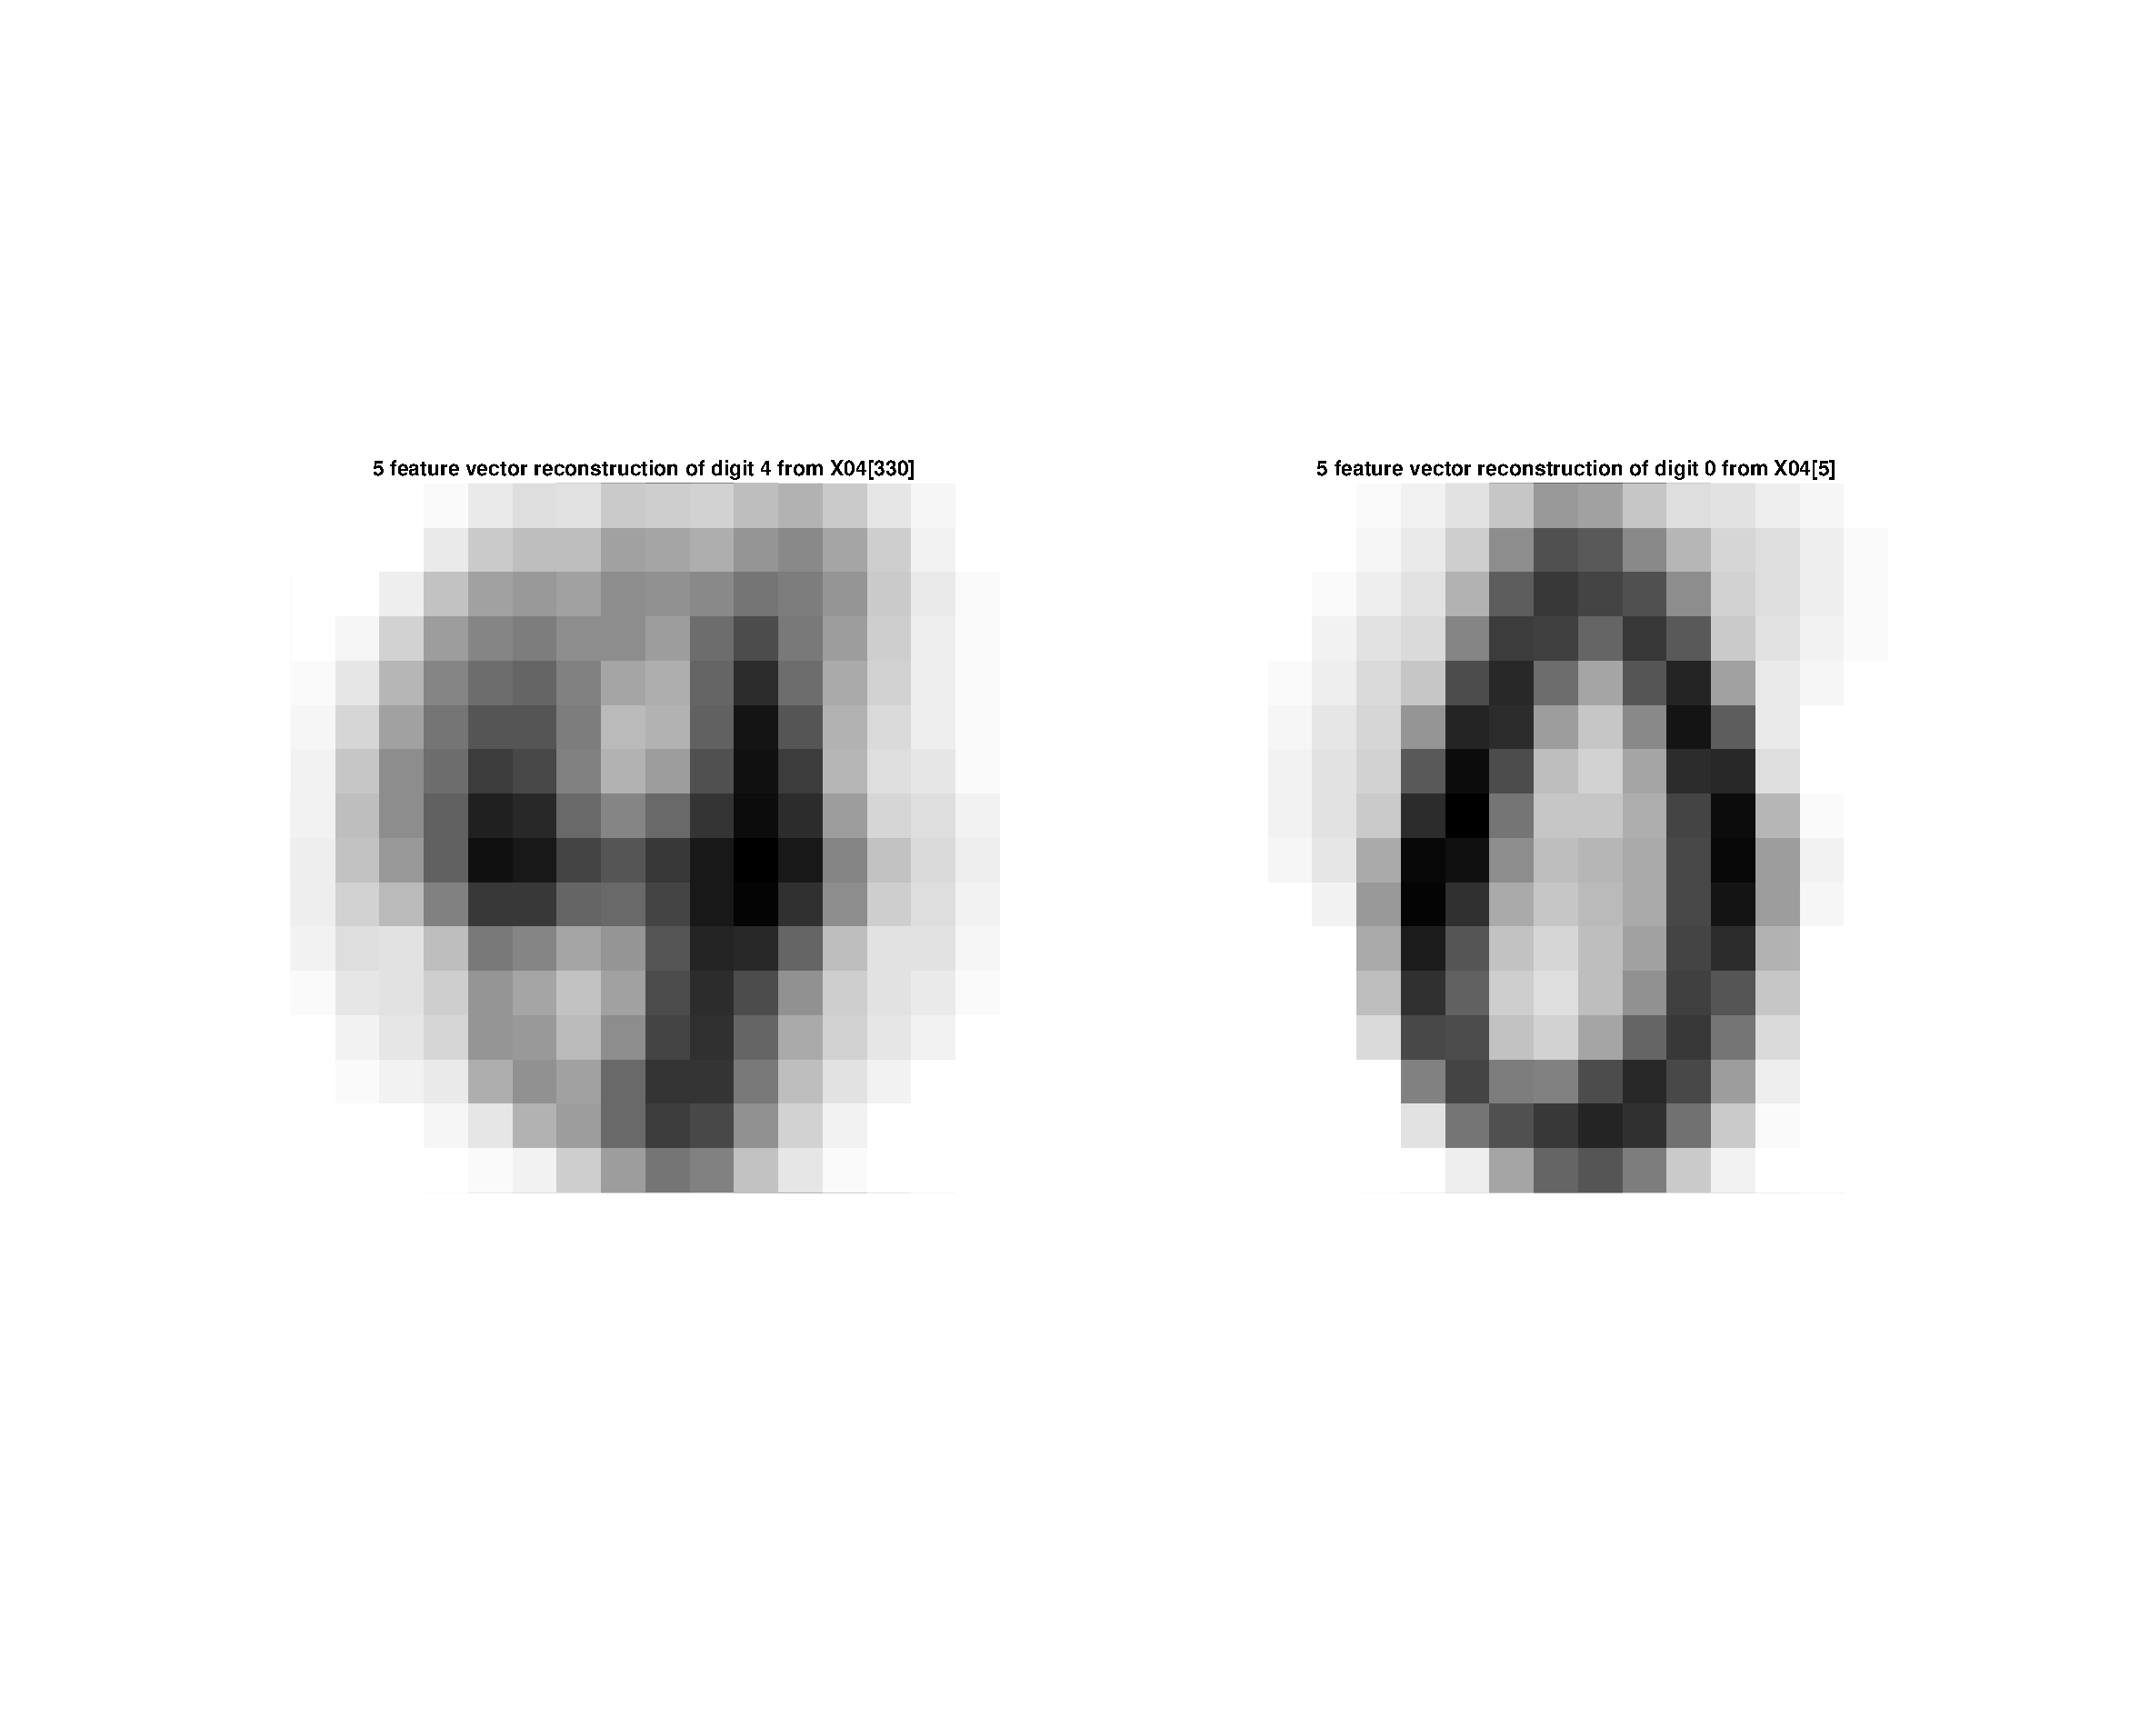
\includegraphics[width=10cm, height=7cm]{Q2_b_reconstructed}
    }
    \caption{\label{fig:my figure}  Reconstruction of 4 (left panel) and 0 (right panel) using W*H and 5 feature vectors.  The 4 is at index 330 in X04 and the 0 at index 5 in X04}
\end{figure}

\begin{figure}[H]
    \centerline
    {
    \includegraphics[width=10cm, height=7cm]{Q2_b_H_values}
    }
    \caption{\label{fig:my figure}  Column Vectors at index 1 and 330 from H.   Each row 1<i<5 within the column vector represents how much we multiply the ith feature by in W. So for column 0, which we know corresponds to a 0, it is appropriate that the H values are high for rows 1,2, and 3 because these correspond to feature vectors 1,2, and 3 which we know are 0's.  And feature vector 4 is a 4, so it is good that H(:,1) has a 0 coefficient for this.  For column 330, we expect a high value at row 4 and lesser values for the other rows, which the data reflects.   }
\end{figure}

\subsubsection*{Analysis}
\textbf{REVISED}
We can see from figures 4, 5, and 6, which plots k=[5,10, 20] feature vectors from W respectively, that indeed some of the feature vectors are clearly representing a 0  and some clearly a 4 just as the algorithm should do.  I can verify the robustness of the algorithm by using W and H to reconstruct the images.  I have picked a random 4 (index 330 in X04) and a random 0 (index 5 in X04) and reconstructed them using the coefficients in H and the feature vectors of W.  The results are shown in figure 7, where we have a very well approximated 0 and a decent 4.  It makes sense that the 0 is approximated so well because of the five feature vectors we use to approximate, four of them correspond to a 0, so we have a lot of data to approximate the zero with.  The 4 is approximated worse because of the five feature vectors we approximate with, only one corresponds to a 4, so the approximation is rougher.  
\\
I will lastly analyze the columns of H to show how it reflects the data.  H stores coefficients for each feature vector in W that tell us how strongly that feature vector composes a data point.  For instance, if a feature vector clearly represents a 0 and the corresponding H is high, then we know that the data vector is likely a 0.  So, When k=5, we see that feature vectors 1,2,3, and 5 correspond to 0 and feature vector 3 corresponds to a 4.  This means that for a 0 image (say at index j), the column vector of H at j should have high indices for rows 1,2,3, and 5, and a low index for row 4.  We know that the first 319 images are 0 and the last 122 are 4, so when I look at the 3rd row for the first 319 images most of the values are 0 or close to it.  And after 319 the 3rd row is never 0, which is exactly what we want.  To do a more case analysis, I will analyze the same images that we reconstructed earlier. The zero image comes from index 1 in X04 an the 4 image from index 330 in X04.  The column vectors in H for the two images are shown in figure(8).  The 0 image has larger coefficients corresponding to feature vectors 1,2, and 3 as expected, since those feature vectors produce a 0.  And for the 4 image, we expect a large coefficient at row 4 because feature vector 4 corresponds to a 4, which the data reflects.
\pagebreak

\pagebreak
\section*{Appendix 1: LDA.mat Matlab Code}
\begin{verbatim}
    function [V,D] = LDA(X,I)
[n,p]=size(X);  

% x_c=zeros(n,1);
% x_c=(1/p)*(sum(X(:,1:p),2));
% X(:,1:p)=X(:,1:p)-x_c(:);


num_clusters=size(unique(I),1);
cluster_vals=unique(I);

I_c = cell(num_clusters,2);

for i = 1:num_clusters
    I_cur = find(I==cluster_vals(i));   
    I_c{i,1} = I_cur;     
    I_c{i,2}=size(I_cur,1);
end

%define annotation vectors
%calculate global centroid and cluster centroids store in c.  col 1=1st,
%2=2nd, 3=3rd, 4=global
c=zeros(n,num_clusters+1);
c(:,num_clusters+1)=(1/size(I,1)) * sum(X(:,:),2);
for i=1:num_clusters
  c(:,i)=(1/I_c{i,2}) * sum(X(:,I==i),2);
end

%center X by its clusters.  Within cluster centered data matrix
X_w=zeros(n,p);
for i=1:num_clusters
    X_w(:,I==cluster_vals(i))=X(:,I==cluster_vals(i))-c(:,i);
end

%Find within cluster scatter matrix Sw
sw=X_w(:,:)*X_w(:,:)';

%Find between cluster scatter matrix
sb=zeros(n,n);
for i=1:num_clusters
    sb=sb+I_c{i,2}*(c(:,i)-c(:,num_clusters+1))*(c(:,i)-c(:,num_clusters+1))';
end

%calculate eigenvalues and eigenvectors
epsilon=10^-12;
sw=sw+(epsilon*eye(n));
[V,D]=eigs(sw\sb,2);
V=real(V);  D=real(D);

figure(1)
colors=['r','g', 'b', 'k'];
for i=1:num_clusters
    Z=V'*X(:,I==cluster_vals(i));
    scatter(Z(1,:),Z(2,:),colors(i));
    xlabel('LDA direction 1');
    ylabel('LDA direction 2');
    title('Plot of LDA direction 1 vs 2 for uncentered Handwritten Dights 0 and 4 ');
    hold on
end
\end{verbatim}

\pagebreak
\section*{Appendix 2: Problem 1 Matlab code}(Call to LDA on wine data)
\begin{verbatim}
load 'WineData.mat'
[V,D]=LDA(X,I);
\end{verbatim}

\pagebreak
\section*{Appendix 3: Problem 2.a Matlab code}(Call to LDA on handwritten digits data)
\begin{verbatim}
load ('HandwrittenDigits.mat')

%define annotation vectors
I04=[I(find(I==0)) I(find(I==4))]';

X04=[X(:,find(I==0)) X(:,find(I==4))];

[V,D]=LDA(X04,I04);
\end{verbatim}


\pagebreak
\section*{Appendix 4: ANLS.mat Matlab Code}
\begin{verbatim}
function [W_new, H_new]= ANLS(X,k)

%initialize W, tolerance, and time
[n,p]=size(X);
W_old=rand(256,k);
H_old=zeros(k,441);
time=0;
t=.001;
dq=1.1;

while dq>t
    %update H 
    H_new=zeros(k,p);
    for j=1:p 
        H_new(:,j)=lsqnonneg(W_old,X(:,j));
    end
    
    %update w
    for i=1:n
        W_new(i,:)=lsqnonneg(H_new',X(i,:)')';
    end
    
    %Calculate norms and scale the matrices
    L=zeros(k,k);
    for i=1:k
        L(i,i)=max(W_new(:,i));
    end
    
    %prepare next iteration
    W_new=W_new*inv(L);
    H_new=L*H_new;
    
    
    w_num=norm(W_new-W_old,'fro');
    w_denom=norm(W_old, 'fro');
    h_num=norm(H_new-H_old, 'fro');
    h_denom=norm(H_old, 'fro');
    
    H_old=H_new;
    W_old=W_new;

    dw=w_num/w_denom;
    dh=h_num/h_denom;    
    dq=dh+dw;
    time=time+1;   

end
end
\end{verbatim}

\pagebreak
\section*{Appendix 5: Problem 2.b Matlab code}(Call to ANLS on handwritten digits data)
\begin{verbatim}
load ('HandwrittenDigits.mat')

K=[5,10,20];
%define annotation vectors and X04 matrix
I_0=find(I==0);
I_4=find(I==4);
X04=[X(:,I_0) X(:,I_4)];

time=1;
for i=1:3
    k=K(i);
    [W_new, H_new]=ANLS(X04,k);
    figure(i)
    for j=1:k
        subplot(5,4,j)
        imagesc(reshape(W_new(:,j),16,16)');
        colormap(1-gray);
        axis('square');
        axis('off');
        title(['#' num2str(j) ' feature vector of ' num2str(k) ' feature vector ANLS analysis of digits 0 and 4'])
    end
    
    figure(100*time)
    subplot(1,2,1)
    imagesc(reshape(W_new*H_new(:,330),16,16)');
    colormap(1-gray);
    axis('square');
    axis('off');
    title([num2str(k) ' feature vector reconstruction of digit 4 from X04[330]' ])
    
    subplot(1,2,2)
    imagesc(reshape(W_new*H_new(:,5),16,16)');
    colormap(1-gray);
    axis('square');
    axis('off');
    title([num2str(k) ' feature vector reconstruction of digit 0 from X04[5]' ])
    
    
    time=time+1;
end
\end{verbatim}


\end{document}
